
\documentclass[table]{eecslides}

% \usecolortheme{RimouskiDark}

\usepackage{lmodern}

\usepackage{scrextend}
\changefontsizes{8.5pt}

\usepackage[english]{babel}
\usepackage{lipsum}

\usepackage{hyperref}
\usepackage{xcolor}
\usepackage[round,authoryear]{natbib}
\usepackage[protrusion=true,expansion=true]{microtype}
\usepackage{xcolor}
\usepackage{tabularx}
\usepackage{bookman}
\usepackage{pgfplots}
\usepackage{pgfplotstable}
\usepackage{tikz}
\usepackage{graphicx}
\usepackage{caption}
\usepackage{mathpazo}

\definecolor{brewforest1}{RGB}{65,171,93}
\definecolor{brewforest2}{RGB}{161,217,155}
\definecolor{brewforest3}{RGB}{49,163,84}


\setlength{\extrarowheight}{3pt}

\title[]{Role of alternative stable states on Sugar maple range shift in reaction to climate change.}
\author[]{\color{white}  Steve Vissault}
\website{\color{white} \textit{s.vissault@yahoo.fr}}
\institute[\color{white} UQAR]{\color{white} \textbf{Research proposal \\
Université du Québec à Rimouski}}
\date{ \color{white} \today}

\setbeamersize{text margin left=1cm}
\setbeamersize{text margin right=1cm}
\setbeamersize{text margin top=0.1cm}

\begin{document}

\begin{frame}[plain]
	\titlepage
\end{frame}

\begin{frame}[plain]{Table of content}{Master proposal presentation}
\tableofcontents
\end{frame}

%%%%%%%%%%%%%%%%
\section{Introduction}
%%%%%%%%%%%%%%%%

\begin{frame}{Introduction}{Sugar maple: a valuable species}
	\begin{column}{.3\paperwidth}
		\begin{figure}
			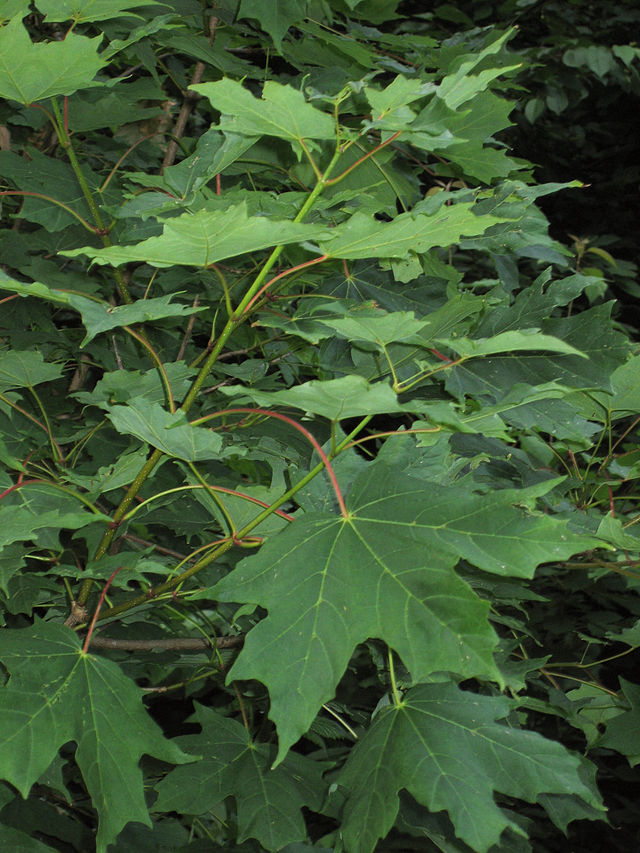
\includegraphics[width=.30\paperwidth]{Figs/Acer.jpg}
			\caption*{}
		\end{figure}
	\end{column}
	\begin{column}{.5\paperwidth}
	\textbf{\alert{Sugar maple}}
		\begin{description}
			\item[Family] Sapindaceae
			\item[Genus] \textit{Acer}
			\item[Species] \textit{saccharum}
		\end{description}
	\pause
	\vspace{1em}
	\textbf{Prime economic importance} in many regions of Quebec
	(e.g hardwood harvesting, syrup producer)
	\end{column}
\end{frame}


%%%%%%%%%%%%%%%%%%%%%%%%%%%%%%%%%%%%%%%%%%%%%%%%%%%

\begin{frame}{Introduction}{The boreal-temperate forest ecotone}
	\begin{figure}
		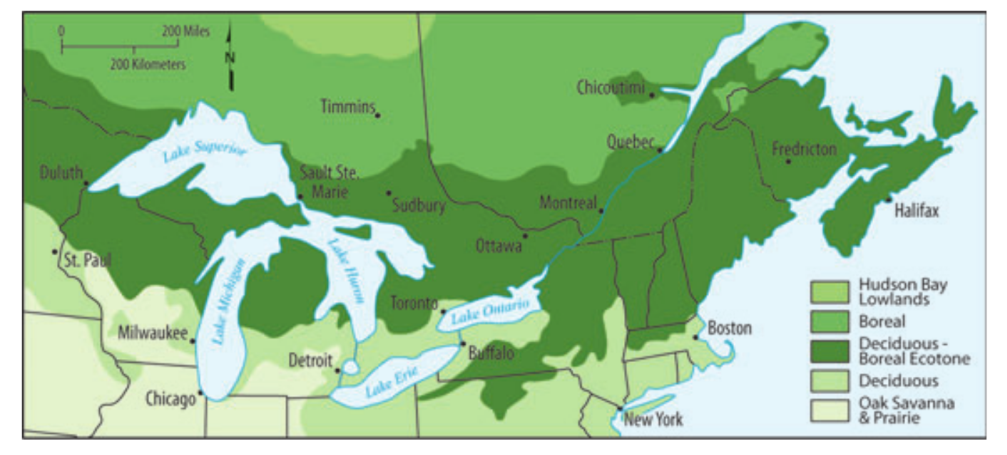
\includegraphics[width=.6\paperwidth]{Figs/ecotone.pdf}
		\caption*{\scriptsize{\cite{Goldblum2010}}}
	\end{figure}

\begin{center}
	Northern range limit of \textbf{Sugar maple} corresponds to the \textbf{upper boundary of the ecotone}.\\
\end{center}

%  L'érable se situe à limite nord de l'écotone entre la forêt boréal et la forêt temprérée nordiques
% Un écotone est reconnue comme étant particulièrement sensible aux changements climatiques

\end{frame}


%%%%%%%%%%%%%%%%%%%%%%%%%%%%%%%%%%%%%%%%%%%%%%%%%%%

\begin{frame}{Introduction}{Sugar maple range shift}

\begin{columns}[c]
	\begin{column}{.4\paperwidth}
		\begin{figure}
			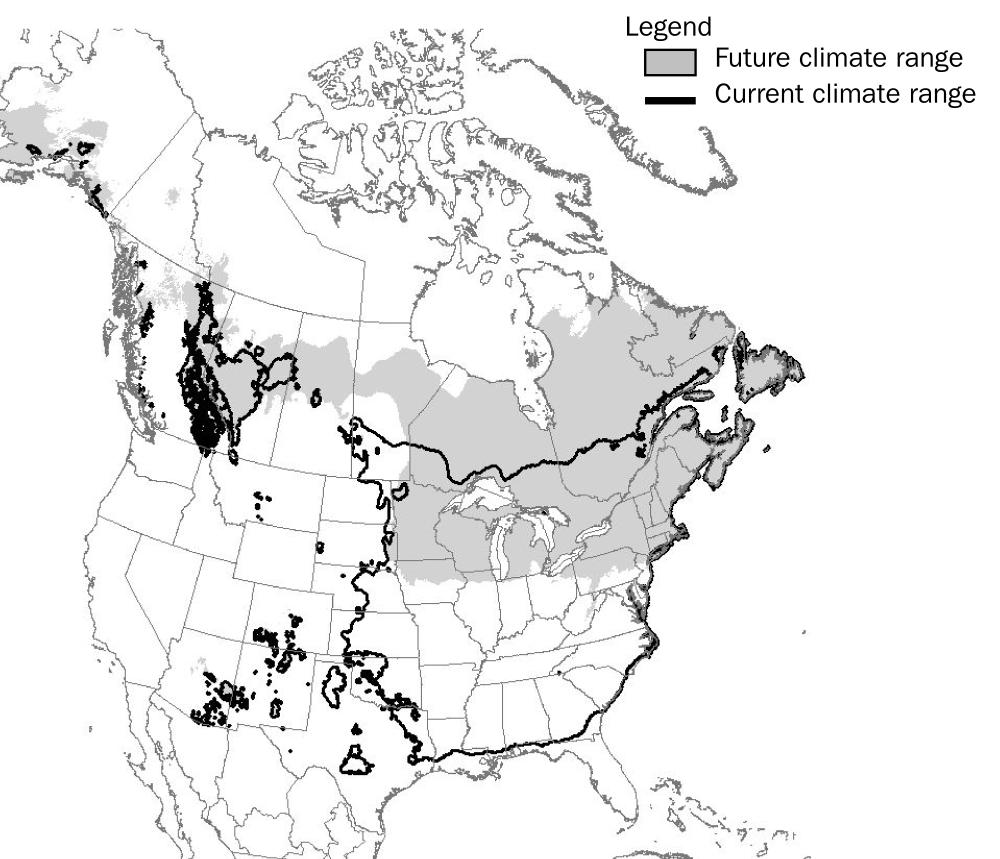
\includegraphics[width=.45\paperwidth]{Figs/sugar_map_distrib.jpg}
			\caption*{\scriptsize{\cite{Sciences2014}}}
		\end{figure}
	\end{column}
	\begin{column}{.5\paperwidth}
		 \begin{itemize}
		  \item Distribution of maple sugar is coming to shift northward
		  \item Reach the Ungava bay within the next 100 years
		 \end{itemize}
		  \pause
		  \vspace{1em}
		  \textbf{Highly improbable: }
		  \begin{enumerate}
		  	\item Dispersal limitations
		  	\item Slow population dynamic
		  	\item SDMs accounting only climatic conditions
		  \end{enumerate}

	\end{column}
\end{columns}

\end{frame}


%%%%%%%%%%%%%%%%%%%%%%%%%%%%%%%%%%%%%%%%%%%%%%%%%%%

\begin{frame}{Introduction}{Difficult transition for Sugar maple}

Sugar maple regeneration depends both on
macro (i.e. regional climate) and \textbf{micro environmental conditions} (i.e. soil)

%\pause
%\begin{columns}[c]
%	\begin{column}{.40\paperwidth}
%		\begin{figure}
%			\caption*{\textbf{\alert{Boreal forest soil}}}
%			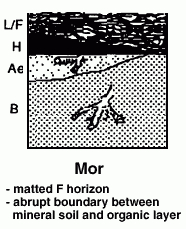
\includegraphics[width=.20\paperwidth]{Figs/mor.jpg}
%		\end{figure}
%	\end{column}
%	\begin{column}{.40\paperwidth}
%		\begin{figure}
%			\caption*{\textbf{\alert{Northern temperate forest soil}}}
%			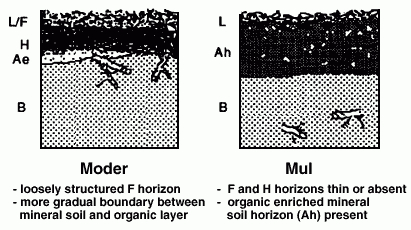
\includegraphics[width=.42\paperwidth]{Figs/moder_mull.jpg}
%		\end{figure}
%	\end{column}
%\end{columns}

\pause
\begin{columns}[c]
	\begin{column}{.40\paperwidth}
		\begin{figure}
			\caption*{\textbf{Boreal forest}}
			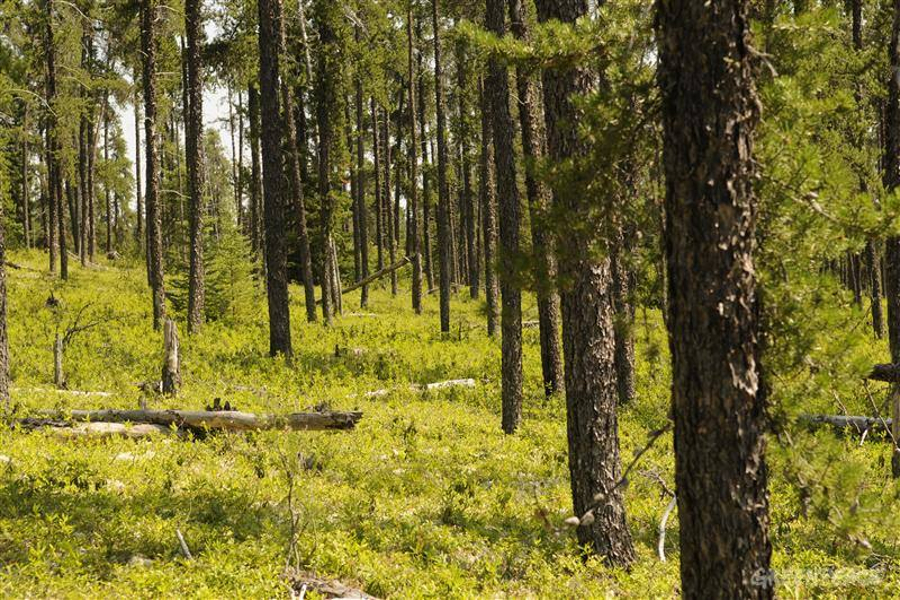
\includegraphics[width=.40\paperwidth]{Figs/bor_forest.jpg}
		\end{figure}
	\end{column}
	\begin{column}{.40\paperwidth}
		\begin{figure}
			\caption*{\textbf{Northern temperate forest}}
			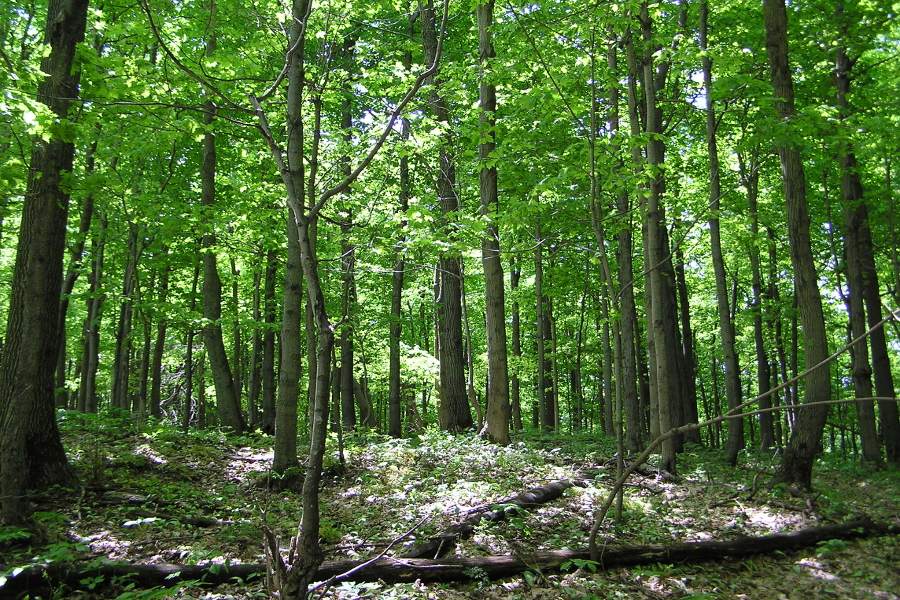
\includegraphics[width=.40\paperwidth]{Figs/temp_forest2.jpg}
		\end{figure}
	\end{column}
\end{columns}
\end{frame}

%%%%%%%%%%%%%%%%%%%%%%%%%%%%%%%%%%%%%%%%%%%%%%%%%%%

\begin{frame}[t]{Introduction}{Difficult transition for Sugar maple}
\vspace{-1.5em}
\begin{columns}[c]
	\begin{column}{.40\paperwidth}
		\begin{figure}
			\caption*{\textbf{Boreal forest}}
			\vspace{-0.5em}
			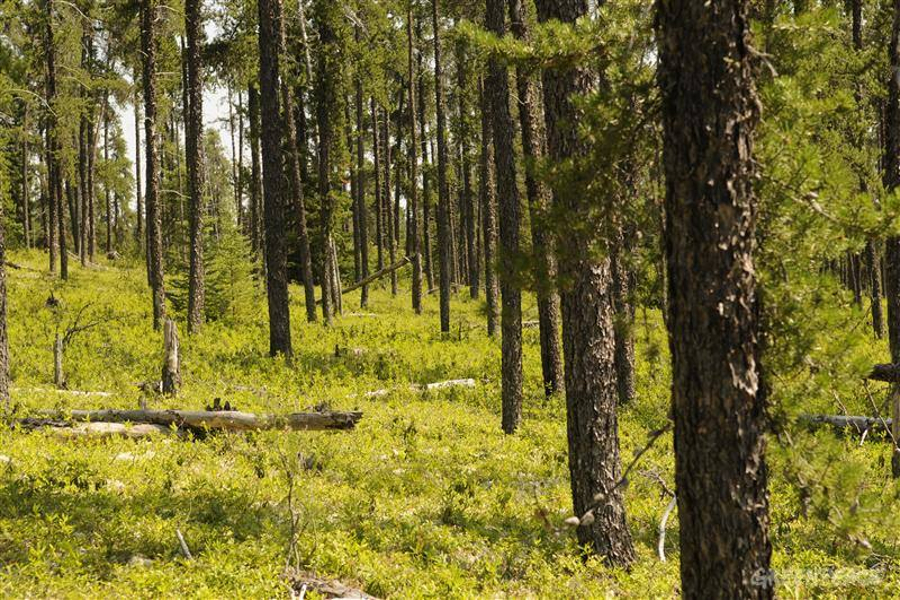
\includegraphics[width=.30\paperwidth]{Figs/bor_forest.jpg}
		\end{figure}
	\end{column}
	\begin{column}{.40\paperwidth}
		\begin{figure}
			\caption*{\textbf{Northern temperate forest}}
			\vspace{-0.5em}
			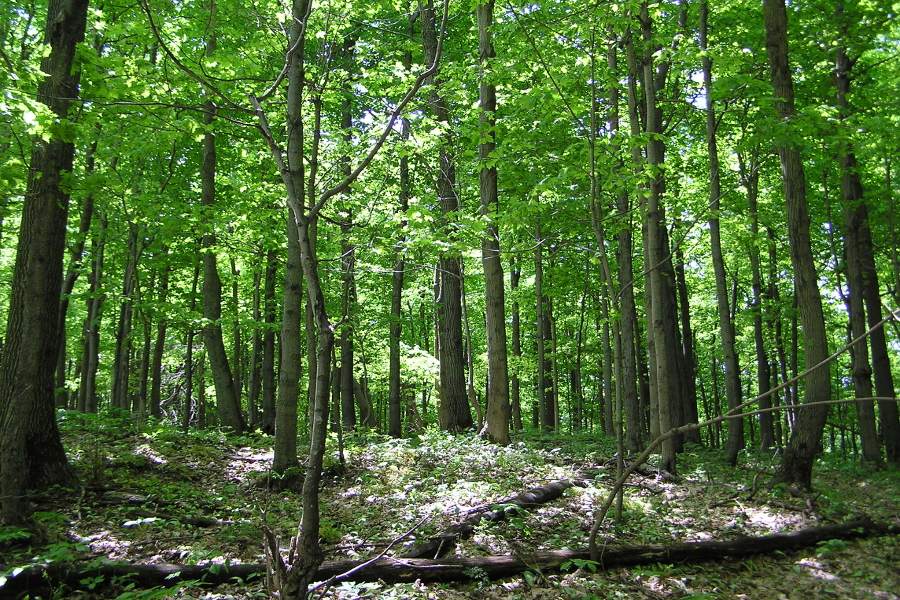
\includegraphics[width=.30\paperwidth]{Figs/temp_forest2.jpg}
		\end{figure}
	\end{column}
\end{columns}
\vspace{-1em}
\begin{columns}[c]
	\begin{column}{.40\paperwidth}
		\begin{figure}
			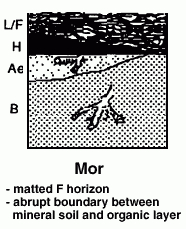
\includegraphics[width=.20\paperwidth]{Figs/mor.jpg}
		\end{figure}
	\end{column}
	\begin{column}{.40\paperwidth}
		\begin{figure}
			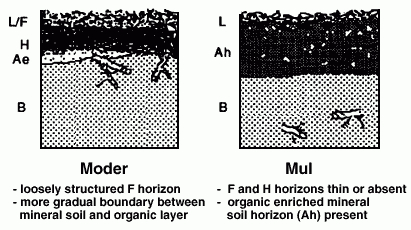
\includegraphics[width=.42\paperwidth]{Figs/moder_mull.jpg}
		\end{figure}
	\end{column}
\end{columns}

\footnotesize {\cite{Lavender1990}}
\end{frame}

%%%%%%%%%%%%%%%%%%%%%%%%%%%%%%%%%%%%%%%%%%%%%%%%%%%

\begin{frame}{Introduction}{The boreal-temperate forest ecotone}
	\begin{figure}
		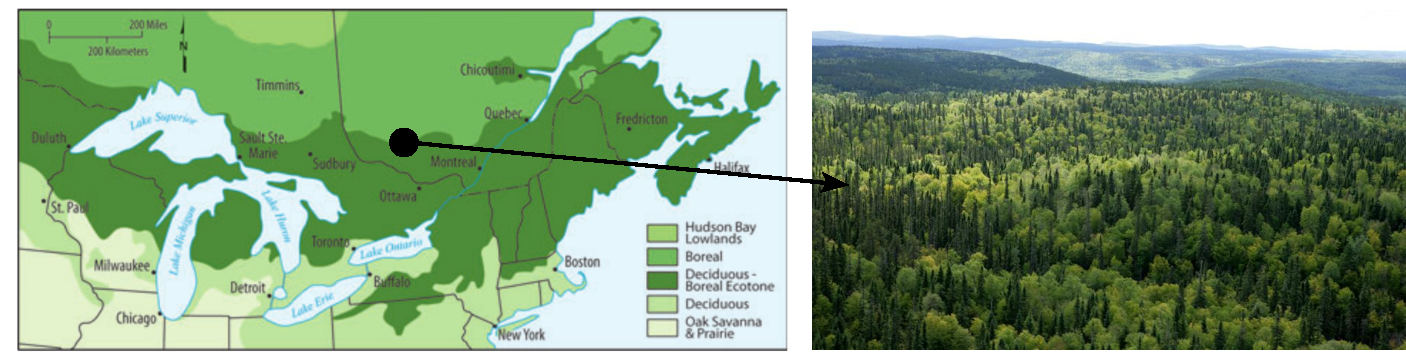
\includegraphics[width=.85\paperwidth]{Figs/ecotone_structure.pdf}
		\caption*{\scriptsize{\cite{Goldblum2010}}}
	\end{figure}

	\begin{center}
		Moisaic landscape structured by the species community, where Sugar maple are present in the northern temperate forest. \\
	\end{center}
\end{frame}

%%%%%%%%%%%%%%%%
\section{Objective \& H_{1-2}}
%%%%%%%%%%%%%%%%
%%%%%%%%%%%%%%%%%%%%%%%%%%%%%%%%%%%%%%%%%%%%%%%%%%%

\begin{frame}{The study}{Objective and hypotheses}

\textbf{Main objective:} Investigate the role of alternative stable states in the transition between the boreal and
temperate forests under different climate change scenarios.

\pause
\vfill

\textbf{Specific hypotheses: }

\begin{description}
	\item [$H_1$] Alternative stable states do co-occur at the boreal-temperate forests ecotone
	\pause
	\item [$H_2$] Response of Sugar maple to climate change will be delayed in areas where alternative stable states are susceptible to occur
\end{description}

\end{frame}

%%%%%%%%%%%%%%%%%%%%%%%%%%%%%%%%%%%%%%%%%%%%%%%%%%%

\begin{frame}{The study}{Objective and hypotheses}

\textbf{Main objective:} Investigate the role of \alert{\textbf{alternative stable states}} in the transition between the boreal and
temperate forests under different climate change scenarios.

\vfill

\textbf{Specific hypotheses: }

\begin{description}
	\item [$H_1$] \alert{\textbf{Alternative stable states}} do co-occur at the boreal-temperate forests ecotone
	\item [$H_2$] Response of Sugar maple to climate change will be delayed in areas where \alert{\textbf{alternative stable states}} are susceptible to occur
\end{description}

\end{frame}

%%%%%%%%%%%%%%%%
\section{Review}
%%%%%%%%%%%%%%%%

\begin{frame}{Review}{Alternative stable states}

According to \cite{scheffer2009critical}, alternative stable states mean a \textbf{contrasting states} to which a system may converge \textbf{under same external condition}

\end{frame}

%%%%%%%%%%%%%%%%%%%%%%%%%%%%%%%%%%%%%%%%%%%%%%%%%%%

\begin{frame}{Review}{Alternative stable states}

\begin{center}
	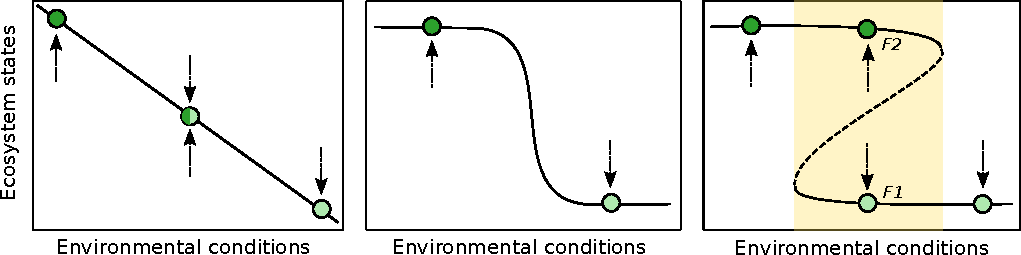
\includegraphics[width=.7\paperwidth]{Figs/ass1.pdf}\\
	\vfill
	\pause
	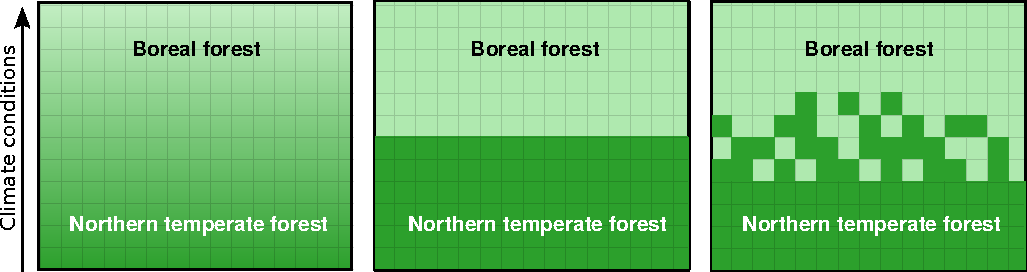
\includegraphics[width=.7\paperwidth]{Figs/ass2.pdf}
\end{center}

\end{frame}

%%%%%%%%%%%%%%%%
\section{State and Transitional Model}
%%%%%%%%%%%%%%%%
%%%%%%%%%%%%%%%%%%%%%%%%%%%%%%%%%%%%%%%%%%%%%%%%%%%
\begin{frame}[t]{Methods}
	\textbf{The Hypotheses: }
	\begin{description}
		\item [$H_1$] \alert{\textbf{Alternative stable states}} do co-occur at the boreal-temperate forests ecotone
		\item [$H_2$] Response of Sugar maple to climate change will be delayed in areas where \alert{\textbf{alternative stable states}}are susceptible to occur
	\end{description}
\textbf{Which tool will be used to answer those hypotheses ?}
\end{frame}
%%%%%%%%%%%%%%%%%%%%%%%%%%%%%%%%%%%%%%%%%%%%%%%%%%%

%%%%%%%%%%%%%%%%
\subsection{Model presentation}
%%%%%%%%%%%%%%%%

\begin{frame}[t]{Methods}{State and Transitional Model}

\textbf{We will use a State and Transitional Model (STM)}

\vspace{-1.5em}
\begin{columns}[c]
	\begin{column}[c]{.40\paperwidth}
		\begin{figure}
			\small{\begin{center}

\tikzstyle{noeud}=[circle,
    thick,
    minimum size = 1.5cm,
    inner sep =5pt,
    draw=brewforest3,
    fill=brewforest1]
\tikzstyle{noeud2}=[circle,
    thick,
    minimum size = 1cm,
    inner sep =5pt,
    draw=brewforest3,
    fill=brewforest3]
\tikzstyle{noeud3}=[circle,
    thick,
    minimum size = 1.5cm,
    inner sep =5pt,
    draw=brewforest3,
    fill=brewforest3]

\begin{tikzpicture}[->,>=stealth',auto,scale=0.45]
    \node [circle,noeud2] (M) at (0,0) {\color{white}\textbf{M}};
    \node [circle,noeud2] (C) at (-5,5) {\color{white}\textbf{C}};
    \node [circle,noeud2] (D) at (5,5) {\color{white}\textbf{D}};
    \node [circle,noeud2] (T) at (0,10) {\color{white}\textbf{T}};

    \draw[thick,-latex] (M) to[bend right=10] node[above,sloped] {} (C);
    \draw[thick,-latex] (C) to[bend right=10] node[below,sloped] {} (M);

    \draw[thick,-latex] (D) to[bend right=10] node[above,sloped] {} (M);
    \draw[thick,-latex] (M) to[bend right=10] node[below,sloped] {} (D);

    \draw[thick,-latex] (D) to[bend right=10] node[above,sloped] {} (T);
    \draw[thick,-latex] (T) to[bend right=10] node[below,sloped] {} (D);

    \draw[thick,-latex] (T) to[bend right=10] node[above,sloped] {} (C);
    \draw[thick,-latex] (C) to[bend right=10] node[below,sloped] {} (T);

    \draw[thick,-latex,transform canvas={xshift=0.6ex}] (T) to node[above,sloped,rotate=90,transform canvas={xshift=1.5ex}] {} (M);
    \draw[thick,-latex,transform canvas={xshift=-0.6ex}] (M) to node[above,sloped,rotate=-90,transform canvas={xshift=-1.5ex}] {} (T);
\end{tikzpicture}
\end{center}

}
		\end{figure}
	\end{column}
	\begin{column}[l]{.40\paperwidth}
		\begin{itemize}
			\item Lanscape modelling scale
			\item 4 States (C,D,M,T)
			\item T correspond to a post-disturbance patch
			\item Probability of transition given climatic conditions
			\item Discrete time and stochastic model
		\end{itemize}
	\end{column}
\end{columns}

\end{frame}

%%%%%%%%%%%%%%%%%%%%%%%%%%%%%%%%%%%%%%%%%%%%%%%%%%%

\begin{frame}[t]{Methods}{State and Transitional Model}

\textbf{We will use a State and Transitional Model (STM)}
\vspace{-1.5em}
\begin{columns}[c]
	\begin{column}[c]{.40\paperwidth}
		\begin{figure}
			\small{\begin{center}

\tikzstyle{noeud}=[circle,
	thick,
	minimum size = 1.5cm,
	inner sep =5pt,
	draw=brewforest3,
	fill=brewforest1]
\tikzstyle{noeud2}=[circle,
	thick,
	minimum size = 1cm,
	inner sep =5pt,
	draw=brewforest3,
	fill=brewforest3]
\tikzstyle{noeud3}=[circle,
	thick,
	minimum size = 1.5cm,
	inner sep =5pt,
	draw=brewforest3,
	fill=brewforest3]

\begin{tikzpicture}[->,>=stealth',auto,scale=0.45]
	\node [circle,noeud2] (M) at (0,0) {\color{white}\textbf{M}};
	\node [circle,noeud2] (C) at (-5,5) {\color{white}\textbf{C}};
	\node [circle,noeud2] (D) at (5,5) {\color{white}\textbf{D}};
	\node [circle,noeud2] (T) at (0,10) {\color{white}\textbf{T}};

	\draw[thick,-latex] (M) to[bend right=10] node[above,sloped] {$\theta_c$} (C);
	\draw[thick,-latex] (C) to[bend right=10] node[below,sloped] {$\beta_d \cdot (D+M)$} (M);

	\draw[thick,-latex] (D) to[bend right=10] node[above,sloped] {$\beta_c \cdot (C+M)$} (M);
	\draw[thick,-latex] (M) to[bend right=10] node[below,sloped] {$\theta_d$} (D);

	\draw[thick,-latex] (D) to[bend right=10] node[above,sloped] {$\epsilon$} (T);
	\draw[thick,-latex] (T) to[bend right=10] node[below,sloped] {$\phi_d$} (D);

	\draw[thick,-latex] (T) to[bend right=10] node[above,sloped] {$\phi_c$} (C);
	\draw[thick,-latex] (C) to[bend right=10] node[below,sloped] {$\epsilon$} (T);

	\draw[thick,-latex,transform canvas={xshift=0.6ex}] (T) to node[above,sloped,rotate=90,transform canvas={xshift=1.5ex}] {$\phi_m $} (M);
	\draw[thick,-latex,transform canvas={xshift=-0.6ex}] (M) to node[above,sloped,rotate=-90,transform canvas={xshift=-1.5ex}] {$\epsilon$} (T);
\end{tikzpicture}
\end{center}

}
		\end{figure}
	\end{column}
	\begin{column}[l]{.40\paperwidth}
	\begin{itemize}
		\item $\beta$: Colonization rate\\
		\item $\theta$: Succession rate\\
		\item $\phi$: Regeneration functions\\
		\item $\epsilon$: Disturbance rate.
	\end{itemize}
	\vspace{1em}
	Each rate depends:
		\begin{itemize}
			\item Proportion of states available in the system
			\item Climatic conditions encounter by the patch
		\end{itemize}
	\end{column}
\end{columns}

\end{frame}

%\begin{frame}[t]{Methods}{Hypothesis 1}
%
%\footnotesize{\textbf{$H_1$} Alternative stable states do co-occur at the boreal-temperate forests ecotone}
%
%\vspace{1em}
%
%\textbf{What we expect ?}
%
%%\begin{figure}
%%	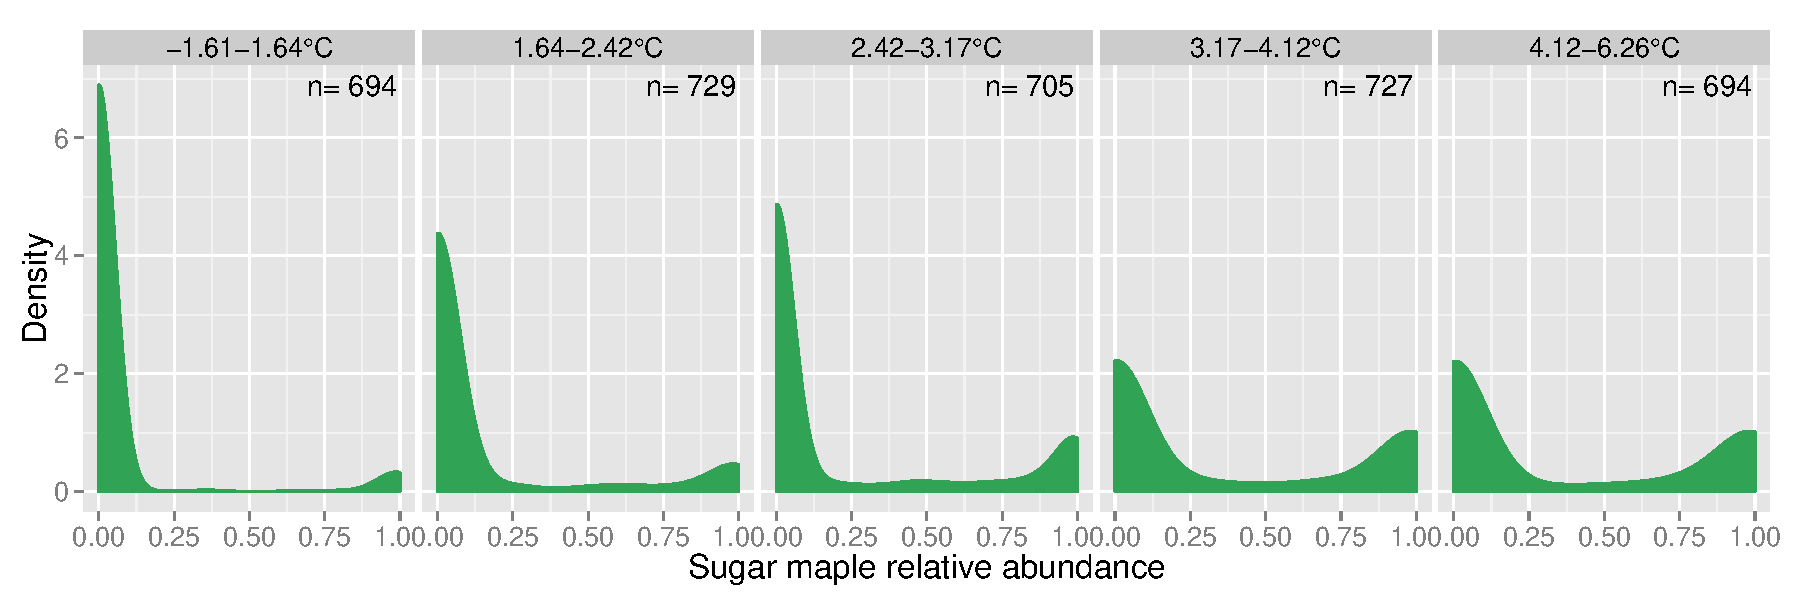
\includegraphics[width=0.85\paperwidth]{Figs/window_temp.pdf}
%%\end{figure}
%
%\end{frame}

%%%%%%%%%%%%%%%%
\subsection{Data}
%%%%%%%%%%%%%%%%
%%%%%%%%%%%%%%%%%%%%%%%%%%%%%%%%%%%%%%%%%%%%%%%%%%%

\begin{frame}{QUICC-FOR}{Data description}

\textbf{Data structure:}
	\begin{itemize}
		\item Permanent and temporary forest inventory sample plots (\textit{ca.} 160,000 plots)
		\item 4 databases (USA,QC, ON, NB)
		\item Started in the 1970s
		\item Interval between sampling ranging from 5 to 10 years
		\item Stem-level information includes diameter at breast height (DBH), species.
		\item Climatic variables are associated to each plot (30 years previous to the year of measurement)
	\end{itemize}

\end{frame}

%%%%%%%%%%%%%%%%%%%%%%%%%%%%%%%%%%%%%%%%%%%%%%%%%%%

\begin{frame}{QUICC-FOR}{Data description}

\textbf{Data filters:}
	\begin{itemize}
		\item 28 representative species of the whole dataset
		\item Only mature stands with dominant strata containing trees greater than 50 years old
		\item Plots with mesic soil conditions
		\item Plots no-disturbed by human activities (mostly by logging)
	\end{itemize}

\end{frame}

%%%%%%%%%%%%%%%%
\subsection{Calibration}
%%%%%%%%%%%%%%%%
%%%%%%%%%%%%%%%%%%%%%%%%%%%%%%%%%%%%%%%%%%%%%%%%%%%

\begin{frame}{Calibration}{1. Plots classification}
Calibration of the model will conduct only on permanent plot\\
\vspace{1em}
\textbf{The first calibration step is the plot classification:}
\vspace{1em}

\begin{table}
\begin{tabular}{|l|l|}
	\hline
	\textbf{States}  & \textbf{Boundaries}\\
	\hline
	D & $Ba_d \geq 75\%$    \\
	C & $Ba_c \geq 75\%$   \\
	M & $Ba_c \geq 25\%$ and $Ba_d \geq 25\%$ \\
	T & $Ba_t  \geq 75\%$ \\
	\hline
\end{tabular}
\end{table}

\end{frame}

%%%%%%%%%%%%%%%%%%%%%%%%%%%%%%%%%%%%%%%%%%%%%%%%%%%

\begin{frame}{Calibration}{2. Compute probability functions}

\textbf{We will compute the probability functions},\\
with as example the transition of a patch D toward M:
\vspace{1em}

\begin{equation}
	P(D_{t1}|M_{t0}, Climate) = f(\overbrace{Climate, \underbrace{\hat{D}, \hat{M}}_\text{Step 1. RandomForest}}^\text{ Step 2. Multinomial regression})
\label{eq1}
\end{equation}
\end{frame}

%%%%%%%%%%%%%%%%%%%%%%%%%%%%%%%%%%%%%%%%%%%%%%%%%%%

\begin{frame}{Calibration}{2. Compute probability functions}

\begin{figure}
	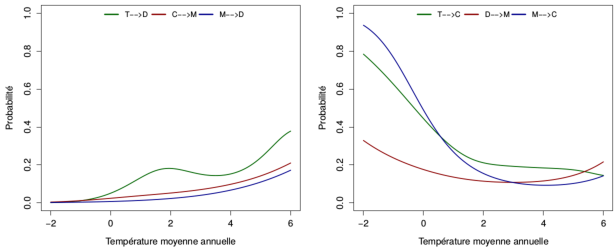
\includegraphics[width=.80\paperwidth]{Figs/Gravel_Bic.pdf}
\end{figure}

\end{frame}

%%%%%%%%%%%%%%%%
\subsection{Validation}
%%%%%%%%%%%%%%%%
%%%%%%%%%%%%%%%%%%%%%%%%%%%%%%%%%%%%%%%%%%%%%%%%%%%

\begin{frame}{Validation}{Cross validation with temporary plots}

\begin{columns}[c]
	\begin{column}[c]{.40\paperwidth}
		\begin{figure}
			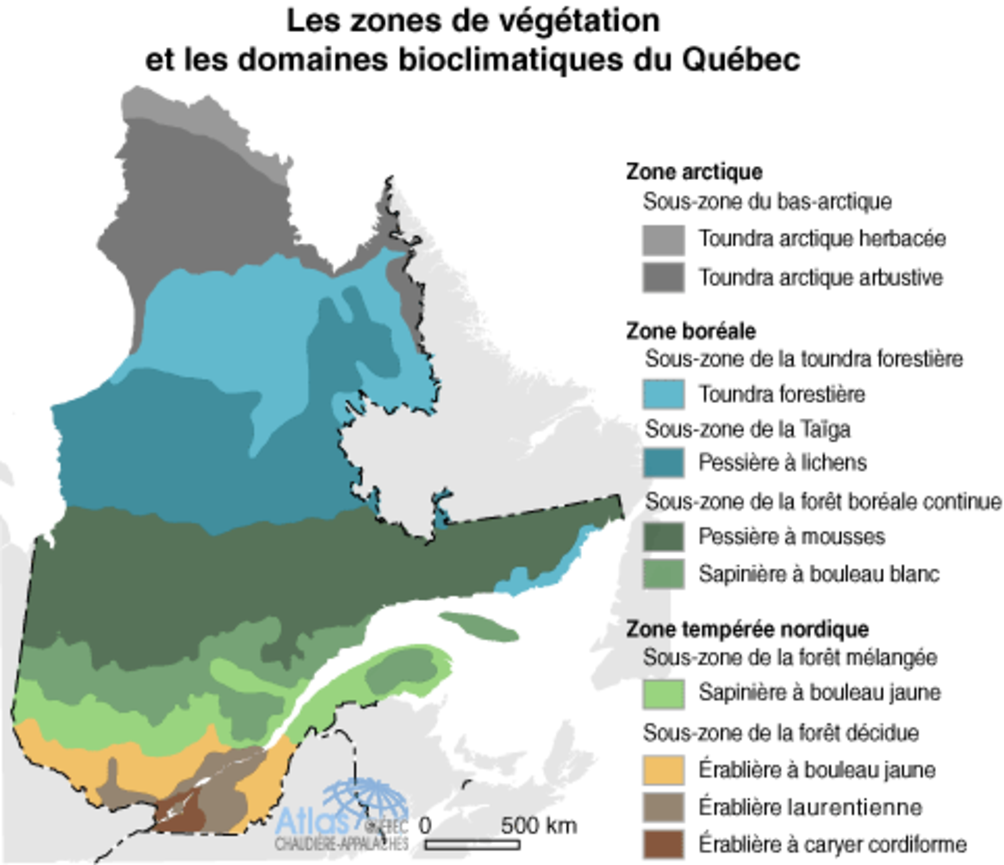
\includegraphics[width=.40\paperwidth]{Figs/zone_vege_qc.pdf}
		\end{figure}
	\end{column}
	\begin{column}[l]{.40\paperwidth}
		\begin{enumerate}
			\item Classify temporary plots into the four states (C,D,M,T)
			\item Compute the states proportion by ecoregions
			\item Run the model previously calibrated
			\item Compare state proportion predicted (PP) to state proportion realized (TP)
		\end{enumerate}
	\end{column}
\end{columns}

\end{frame}


%%%%%%%%%%%%%%%%
\section{Simulation}
%%%%%%%%%%%%%%%%
%%%%%%%%%%%%%%%%%%%%%%%%%%%%%%%%%%%%%%%%%%%%%%%%%%%

\begin{frame}{Simulation}{Hypothesis 1}
$H_1$ Alternative stable states do co-occur at the boreal-temperate forests ecotone
	\begin{figure}
		\caption*{State and Transitional Model}
		\small{\begin{center}

\tikzstyle{noeud}=[circle,
	thick,
	minimum size = 1.5cm,
	inner sep =5pt,
	draw=brewforest3,
	fill=brewforest1]
\tikzstyle{noeud2}=[circle,
	thick,
	minimum size = 1cm,
	inner sep =5pt,
	draw=brewforest3,
	fill=brewforest3]
\tikzstyle{noeud3}=[circle,
	thick,
	minimum size = 1.5cm,
	inner sep =5pt,
	draw=brewforest3,
	fill=brewforest3]

\begin{tikzpicture}[->,>=stealth',auto,scale=0.45]
	\node [circle,noeud2] (M) at (0,0) {\color{white}\textbf{M}};
	\node [circle,noeud2] (C) at (-5,5) {\color{white}\textbf{C}};
	\node [circle,noeud2] (D) at (5,5) {\color{white}\textbf{D}};
	\node [circle,noeud2] (T) at (0,10) {\color{white}\textbf{T}};

	\draw[thick,-latex] (M) to[bend right=10] node[above,sloped] {$\theta_c$} (C);
	\draw[thick,-latex] (C) to[bend right=10] node[below,sloped] {$\beta_d \cdot (D+M)$} (M);

	\draw[thick,-latex] (D) to[bend right=10] node[above,sloped] {$\beta_c \cdot (C+M)$} (M);
	\draw[thick,-latex] (M) to[bend right=10] node[below,sloped] {$\theta_d$} (D);

	\draw[thick,-latex] (D) to[bend right=10] node[above,sloped] {$\epsilon$} (T);
	\draw[thick,-latex] (T) to[bend right=10] node[below,sloped] {$\phi_d$} (D);

	\draw[thick,-latex] (T) to[bend right=10] node[above,sloped] {$\phi_c$} (C);
	\draw[thick,-latex] (C) to[bend right=10] node[below,sloped] {$\epsilon$} (T);

	\draw[thick,-latex,transform canvas={xshift=0.6ex}] (T) to node[above,sloped,rotate=90,transform canvas={xshift=1.5ex}] {$\phi_m $} (M);
	\draw[thick,-latex,transform canvas={xshift=-0.6ex}] (M) to node[above,sloped,rotate=-90,transform canvas={xshift=-1.5ex}] {$\epsilon$} (T);
\end{tikzpicture}
\end{center}

}
	\end{figure}
\end{frame}

\begin{frame}{Simulation}{Hypothesis 2}
$H_2$ Response of Sugar maple to climate change will be delayed in areas where alternative stable states are susceptible to occur
\begin{columns}[c]
	\begin{column}[c]{.40\paperwidth}
		\begin{figure}
			\caption*{State and Transitional Model}
			\small{\begin{center}

\tikzstyle{noeud}=[circle,
	thick,
	minimum size = 1.5cm,
	inner sep =5pt,
	draw=brewforest3,
	fill=brewforest1]
\tikzstyle{noeud2}=[circle,
	thick,
	minimum size = 1cm,
	inner sep =5pt,
	draw=brewforest3,
	fill=brewforest3]
\tikzstyle{noeud3}=[circle,
	thick,
	minimum size = 1.5cm,
	inner sep =5pt,
	draw=brewforest3,
	fill=brewforest3]

\begin{tikzpicture}[->,>=stealth',auto,scale=0.38]
	\node [circle,noeud2] (M) at (0,0) {\color{white}\textbf{M}};
	\node [circle,noeud2] (C) at (-5,5) {\color{white}\textbf{C}};
	\node [circle,noeud2] (D) at (5,5) {\color{white}\textbf{D}};
	\node [circle,noeud2] (T) at (0,10) {\color{white}\textbf{T}};

	\draw[thick,-latex] (M) to[bend right=10] node[above,sloped] {$\theta_c$} (C);
	\draw[thick,-latex] (C) to[bend right=10] node[below,sloped] {$\beta_d \cdot (D+M)$} (M);

	\draw[thick,-latex] (D) to[bend right=10] node[above,sloped] {$\beta_c \cdot (C+M)$} (M);
	\draw[thick,-latex] (M) to[bend right=10] node[below,sloped] {$\theta_d$} (D);

	\draw[thick,-latex] (D) to[bend right=10] node[above,sloped] {$\epsilon$} (T);
	\draw[thick,-latex] (T) to[bend right=10] node[below,sloped] {$\phi_d$} (D);

	\draw[thick,-latex] (T) to[bend right=10] node[above,sloped] {$\phi_c$} (C);
	\draw[thick,-latex] (C) to[bend right=10] node[below,sloped] {$\epsilon$} (T);

	\draw[thick,-latex,transform canvas={xshift=0.6ex}] (T) to node[above,sloped,rotate=90,transform canvas={xshift=1.5ex}] {$\phi_m $} (M);
	\draw[thick,-latex,transform canvas={xshift=-0.6ex}] (M) to node[above,sloped,rotate=-90,transform canvas={xshift=-1.5ex}] {$\epsilon$} (T);
\end{tikzpicture}
\end{center}

}
		\end{figure}
	\end{column}
	\begin{column}[l]{.40\paperwidth}
		\begin{figure}
			\caption*{Cellular automata}
			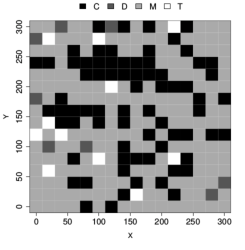
\includegraphics[width=.35\paperwidth]{Figs/Mat_automat.pdf}
		\end{figure}
	\end{column}
\end{columns}
\end{frame}

%%%%%%%%%%%%%%%%
%% References
%%%%%%%%%%%%%%%%

\begin{frame}[allowsframebreaks]{References}
	\scriptsize
	\bibliographystyle{abbrvnat}
	\bibliography{/home/steve/Dropbox/Bibtex/Devis}
\end{frame}

\begin{frame}[plain]
\large{	\textbf{\alert{Thanks for your attention !}}\\
	\vspace{2em}
	Any questions ?}
\end{frame}

\end{document}